\begin{frame}{Beyond ViT Backbones: Point-JEPA and CNN-JEPA}
  \begin{columns}[T,onlytextwidth]
    \column{0.48\textwidth}
    \begin{itemize}\itemsep0.32em
      \item[\textcolor{red}{$\blacktriangleright$}] \textbf{Point-JEPA:} applies the JEPA recipe to \textbf{unordered 3D point sets}; uses spatial proximity and masking in the point domain so the model predicts \textbf{latent structure} of masked regions from geometric context (not pixels).
      \item[\textcolor{red}{$\blacktriangleright$}] \textbf{CNN-JEPA:} keeps \textbf{convolutional} encoders (sparse, translation-friendly) while retaining \textbf{latent prediction} rather than pixel reconstruction---useful when ViTs are not the deployment backbone.
    \end{itemize}
    \column{0.5\textwidth}
    \begin{itemize}\itemsep0.32em
      \item[\textcolor{red}{$\blacktriangleright$}] Related 3D SSL: \textbf{Sonata} (2025) pursues highly reliable point representations from large-scale self-supervision---complementary reading for geometry-heavy applications.
      \item[\textcolor{red}{$\blacktriangleright$}] \textbf{VL-JEPA} extends the same \textbf{predictive latent} philosophy to \textbf{vision--language} setups: build world models that couple visual structure with language for richer situational understanding.
    \end{itemize}
  \end{columns}
\end{frame}

% \begin{frame}{VL-JEPA and Multimodal World Models}
%   \begin{itemize}\itemsep0.3em
%     \item \textbf{VL-JEPA} extends the same \textbf{predictive latent} philosophy to \textbf{vision--language} setups: build world models that couple visual structure with language for richer situational understanding.
%     \item Expository discussion (context, limitations, links to planning): Themesis, ``World Models: JEPA and VL-JEPA,'' \href{https://themesis.com/2026/01/21/world-models-jepa-and-vl-jepa/}{Jan.\ 2026}.
%   \end{itemize}
% \end{frame}

\begin{frame}{Video SSL Efficiency: Frozen Teachers (SALT)}
  \begin{itemize}\itemsep0.3em
    \item[\textcolor{red}{$\blacktriangleright$}] \textbf{SALT} (\emph{Static-teacher Asymmetric Latent Training}, Li et al., 2025) uses a \textbf{two-stage recipe:} (i) train a teacher with a \textbf{pixel reconstruction} objective under V-JEPA--style masking; (ii) \textbf{freeze} the teacher and train a student to predict teacher latents on masked regions.
    \item[\textcolor{red}{$\blacktriangleright$}] Reported benefits: simpler optimization than coupled EMA schedules, favorable \textbf{accuracy--compute} trade-offs in frozen evaluation, and student quality surprisingly robust to teacher size.
  \end{itemize}
\end{frame}

\begin{frame}{SALT: Two-Stage Recipe for Video SSL (Stage 1)}
  \centering
  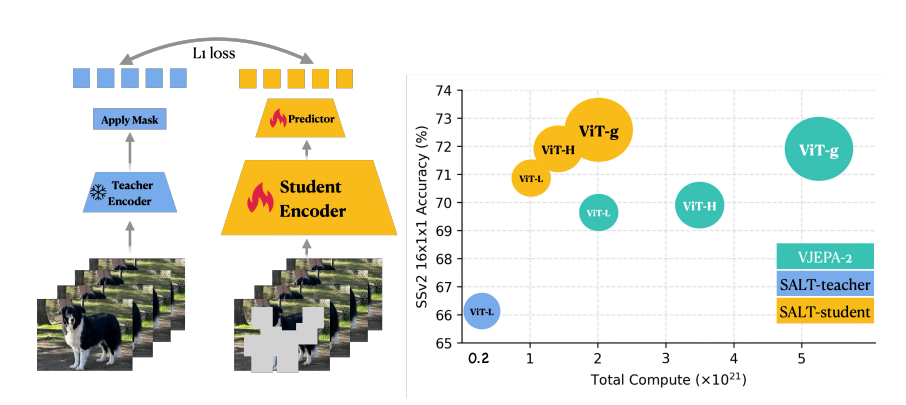
\includegraphics[width=0.99\linewidth, height=0.40\textheight, keepaspectratio]{assets/New-Lecture_JEPA_models/SALT_stages1_2_diagram.png}
  \linebreak
  {\scriptsize Source: Li et al.\ (2025) SALT, \href{https://arxiv.org/pdf/2509.24317}{arXiv:2509.24317}, Fig.\ 2.}
  \begin{itemize}\footnotesize
    \item \textbf{Goal:} Train a \textbf{teacher encoder} to robustly reconstruct masked video regions \emph{at the pixel level}.
    \item \textbf{Approach:} Use a \textbf{V-JEPA-style masking} scheme; teach the encoder to infill missing pixels based on visible context.
    \item\textbf{Outcome:} Teacher encoder learns to summarize temporal and spatial structure, producing feature-rich latent representations.
  \end{itemize}
\end{frame}

\begin{frame}{SALT: Two-Stage Recipe for Video SSL (Stage 2)}
  \centering
  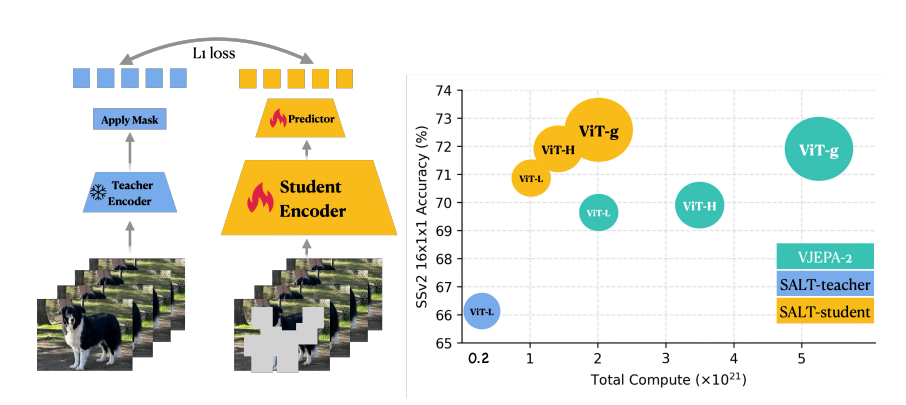
\includegraphics[width=0.99\linewidth, height=0.60\textheight, keepaspectratio]{assets/New-Lecture_JEPA_models/SALT_stages1_2_diagram.png}
  \linebreak
  {\scriptsize Reference: Li et al.\ (2025) SALT, \href{https://arxiv.org/pdf/2509.24317}{arXiv:2509.24317}, Fig.\ 2.}
  \begin{itemize}\footnotesize
    \item \textbf{Freeze} the teacher encoder weights.
    \item Train a student to \textbf{predict teacher latent embeddings} of masked regions, using only visible context as input.
    \item Mimics standard JEPA: loss is in \textbf{latent space}, not directly on pixels.
  \end{itemize}
\end{frame}
